\begin{center}
	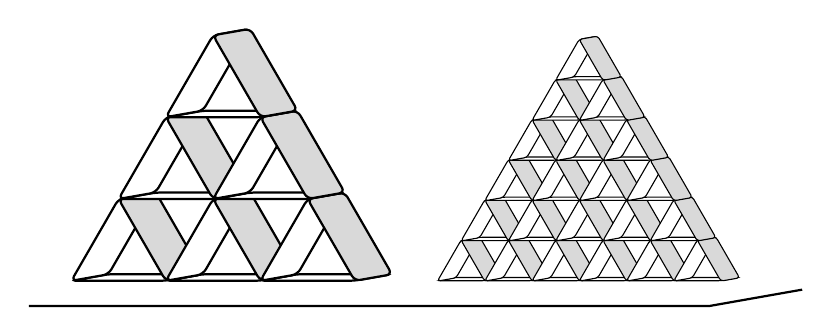
\begin{tikzpicture}[scale = 1.2]
	\draw[thick] (-0.2, -0.2) -- (7, -0.2) -- ++(10:1);
%%%%%% 1 этаж
	\draw[thick, rounded corners = 2, fill = white] (0.75, 0.5*0.136) -- ++(180:0.5) -- ++(10:0.4) -- ++(0:1) -- ++(190:0.4) --cycle;
	\draw[thick, rounded corners = 2, fill = white] (1.75, 0.5*0.136) -- ++(180:0.5) -- ++(10:0.4) -- ++(0:1) -- ++(190:0.4) --cycle;
	\draw[thick, rounded corners = 2, fill = white] (2.75, 0.5*0.136) -- ++(180:0.5) -- ++(10:0.4) -- ++(0:1) -- ++(190:0.4) --cycle;
	\draw[thick, rounded corners = 2, fill = white] (0.5, 0.5) -- ++(60:0.5) -- ++(10:0.4) -- ++(-120:1) -- ++(190:0.4) --cycle;
	\draw[thick, rounded corners = 2, fill = gray!30] (1, 0.5) -- ++(120:0.5) -- ++(10:0.4) -- ++(-60:1) -- ++(190:0.4) --cycle;
	\draw[thick, rounded corners = 2, fill = white] (1.5, 0.5) -- ++(60:0.5) -- ++(10:0.4) -- ++(-120:1) -- ++(190:0.4) --cycle;
	\draw[thick, rounded corners = 2, fill = gray!30] (2, 0.5) -- ++(120:0.5) -- ++(10:0.4) -- ++(-60:1) -- ++(190:0.4) --cycle;
	\draw[thick, rounded corners = 2, fill = white] (2.5, 0.5) -- ++(60:0.5) -- ++(10:0.4) -- ++(-120:1) -- ++(190:0.4) --cycle;
	\draw[thick, rounded corners = 2, fill = gray!30] (3, 0.5) -- ++(120:0.5) -- ++(10:0.4) -- ++(-60:1) -- ++(190:0.4) --cycle;
%%%%%% 2 этаж
	\draw[thick, rounded corners = 2, fill = white] (1.25, 1 - 0.5*0.136) -- ++(180:0.5) -- ++(10:0.4) -- ++(0:1) -- ++(190:0.4) --cycle;
	\draw[thick, rounded corners = 2, fill = white] (2.25, 1 - 0.5*0.136) -- ++(180:0.5) -- ++(10:0.4) -- ++(0:1) -- ++(190:0.4) --cycle;
	\draw[thick, rounded corners = 2, fill = white] (1, 0.5 + 0.866) -- ++(60:0.5) -- ++(10:0.4) -- ++(-120:1) -- ++(190:0.4) --cycle;
	\draw[thick, rounded corners = 2, fill = gray!30] (1.5, 0.5 + 0.866) -- ++(120:0.5) -- ++(10:0.4) -- ++(-60:1) -- ++(190:0.4) --cycle;
	\draw[thick, rounded corners = 2, fill = white] (2, 0.5 + 0.866) -- ++(60:0.5) -- ++(10:0.4) -- ++(-120:1) -- ++(190:0.4) --cycle;
	\draw[thick, rounded corners = 2, fill = gray!30] (2.5, 0.5 + 0.866) -- ++(120:0.5) -- ++(10:0.4) -- ++(-60:1) -- ++(190:0.4) --cycle;
%%%%%% 3 этаж
	\draw[thick, rounded corners = 2, fill = white] (1.75, 1 - 0.5*0.136 + 0.866) -- ++(180:0.5) -- ++(10:0.4) -- ++(0:1) -- ++(190:0.4) --cycle;
	\draw[thick, rounded corners = 2, fill = white] (1.5, 0.5 + 2*0.866) -- ++(60:0.5) -- ++(10:0.4) -- ++(-120:1) -- ++(190:0.4) --cycle;
	\draw[thick, rounded corners = 2, fill = gray!30] (2, 0.5 + 2*0.866) -- ++(120:0.5) -- ++(10:0.4) -- ++(-60:1) -- ++(190:0.4) --cycle;	
%%%%%% 2 домик
%%%%%% 1 этаж
	\draw[rounded corners = 1, fill = white] (4.375, 0.5*0.136) -- ++(180:0.25) -- ++(10:0.2) -- ++(0:0.5) -- ++(190:0.2) --cycle;
	\draw[rounded corners = 1, fill = white] (4.25, 0.5*0.136 + 0.25*0.85) -- ++(60:0.25) -- ++(10:0.2) -- ++(-120:0.5) -- ++(190:0.2) --cycle;
	\draw[rounded corners = 1, fill = gray!30] (4.5, 0.5*0.136 + 0.25*0.85) -- ++(120:0.25) -- ++(10:0.2) -- ++(-60:0.5) -- ++(190:0.2) --cycle;
	\draw[rounded corners = 1, fill = white] (4.875, 0.5*0.136) -- ++(180:0.25) -- ++(10:0.2) -- ++(0:0.5) -- ++(190:0.2) --cycle;
	\draw[rounded corners = 1, fill = white] (4.75, 0.5*0.136 + 0.25*0.85) -- ++(60:0.25) -- ++(10:0.2) -- ++(-120:0.5) -- ++(190:0.2) --cycle;
	\draw[rounded corners = 1, fill = gray!30] (5, 0.5*0.136 + 0.25*0.85) -- ++(120:0.25) -- ++(10:0.2) -- ++(-60:0.5) -- ++(190:0.2) --cycle;
	\draw[rounded corners = 1, fill = white] (5.375, 0.5*0.136) -- ++(180:0.25) -- ++(10:0.2) -- ++(0:0.5) -- ++(190:0.2) --cycle;
	\draw[rounded corners = 1, fill = white] (5.25, 0.5*0.136 + 0.25*0.85) -- ++(60:0.25) -- ++(10:0.2) -- ++(-120:0.5) -- ++(190:0.2) --cycle;
	\draw[rounded corners = 1, fill = gray!30] (5.5, 0.5*0.136 + 0.25*0.85) -- ++(120:0.25) -- ++(10:0.2) -- ++(-60:0.5) -- ++(190:0.2) --cycle;
	\draw[rounded corners = 1, fill = white] (5.875, 0.5*0.136) -- ++(180:0.25) -- ++(10:0.2) -- ++(0:0.5) -- ++(190:0.2) --cycle;
	\draw[rounded corners = 1, fill = white] (5.75, 0.5*0.136 + 0.25*0.85) -- ++(60:0.25) -- ++(10:0.2) -- ++(-120:0.5) -- ++(190:0.2) --cycle;
	\draw[rounded corners = 1, fill = gray!30] (6, 0.5*0.136 + 0.25*0.85) -- ++(120:0.25) -- ++(10:0.2) -- ++(-60:0.5) -- ++(190:0.2) --cycle;
	\draw[rounded corners = 1, fill = white] (6.375, 0.5*0.136) -- ++(180:0.25) -- ++(10:0.2) -- ++(0:0.5) -- ++(190:0.2) --cycle;
	\draw[rounded corners = 1, fill = white] (6.25, 0.5*0.136 + 0.25*0.85) -- ++(60:0.25) -- ++(10:0.2) -- ++(-120:0.5) -- ++(190:0.2) --cycle;
	\draw[rounded corners = 1, fill = gray!30] (6.5, 0.5*0.136 + 0.25*0.85) -- ++(120:0.25) -- ++(10:0.2) -- ++(-60:0.5) -- ++(190:0.2) --cycle;
	\draw[rounded corners = 1, fill = white] (6.875, 0.5*0.136) -- ++(180:0.25) -- ++(10:0.2) -- ++(0:0.5) -- ++(190:0.2) --cycle;
	\draw[rounded corners = 1, fill = white] (6.75, 0.5*0.136 + 0.25*0.85) -- ++(60:0.25) -- ++(10:0.2) -- ++(-120:0.5) -- ++(190:0.2) --cycle;
	\draw[rounded corners = 1, fill = gray!30] (7, 0.5*0.136 + 0.25*0.85) -- ++(120:0.25) -- ++(10:0.2) -- ++(-60:0.5) -- ++(190:0.2) --cycle;
%%%%%% 2 этаж
	\draw[rounded corners = 1, fill = white] (4.875-0.25, 0.5*0.136+0.5*0.85) -- ++(180:0.25) -- ++(10:0.2) -- ++(0:0.5) -- ++(190:0.2) --cycle;
	\draw[rounded corners = 1, fill = white] (4.75-0.25, 0.5*0.136 + 0.25*0.85+0.5*0.85) -- ++(60:0.25) -- ++(10:0.2) -- ++(-120:0.5) -- ++(190:0.2) --cycle;
	\draw[rounded corners = 1, fill = gray!30] (5-0.25, 0.5*0.136 + 0.25*0.85+0.5*0.85) -- ++(120:0.25) -- ++(10:0.2) -- ++(-60:0.5) -- ++(190:0.2) --cycle;
	\draw[rounded corners = 1, fill = white] (5.375-0.25, 0.5*0.136+0.5*0.85) -- ++(180:0.25) -- ++(10:0.2) -- ++(0:0.5) -- ++(190:0.2) --cycle;
	\draw[rounded corners = 1, fill = white] (5.25-0.25, 0.5*0.136 + 0.25*0.85+0.5*0.85) -- ++(60:0.25) -- ++(10:0.2) -- ++(-120:0.5) -- ++(190:0.2) --cycle;
	\draw[rounded corners = 1, fill = gray!30] (5.5-0.25, 0.5*0.136 + 0.25*0.85+0.5*0.85) -- ++(120:0.25) -- ++(10:0.2) -- ++(-60:0.5) -- ++(190:0.2) --cycle;
	\draw[rounded corners = 1, fill = white] (5.875-0.25, 0.5*0.136+0.5*0.85) -- ++(180:0.25) -- ++(10:0.2) -- ++(0:0.5) -- ++(190:0.2) --cycle;
	\draw[rounded corners = 1, fill = white] (5.75-0.25, 0.5*0.136 + 0.25*0.85+0.5*0.85) -- ++(60:0.25) -- ++(10:0.2) -- ++(-120:0.5) -- ++(190:0.2) --cycle;
	\draw[rounded corners = 1, fill = gray!30] (6-0.25, 0.5*0.136 + 0.25*0.85+0.5*0.85) -- ++(120:0.25) -- ++(10:0.2) -- ++(-60:0.5) -- ++(190:0.2) --cycle;
	\draw[rounded corners = 1, fill = white] (6.375-0.25, 0.5*0.136+0.5*0.85) -- ++(180:0.25) -- ++(10:0.2) -- ++(0:0.5) -- ++(190:0.2) --cycle;
	\draw[rounded corners = 1, fill = white] (6.25-0.25, 0.5*0.136 + 0.25*0.85+0.5*0.85) -- ++(60:0.25) -- ++(10:0.2) -- ++(-120:0.5) -- ++(190:0.2) --cycle;
	\draw[rounded corners = 1, fill = gray!30] (6.5-0.25, 0.5*0.136 + 0.25*0.85+0.5*0.85) -- ++(120:0.25) -- ++(10:0.2) -- ++(-60:0.5) -- ++(190:0.2) --cycle;
	\draw[rounded corners = 1, fill = white] (6.875-0.25, 0.5*0.136+0.5*0.85) -- ++(180:0.25) -- ++(10:0.2) -- ++(0:0.5) -- ++(190:0.2) --cycle;
	\draw[rounded corners = 1, fill = white] (6.75-0.25, 0.5*0.136 + 0.25*0.85+0.5*0.85) -- ++(60:0.25) -- ++(10:0.2) -- ++(-120:0.5) -- ++(190:0.2) --cycle;
	\draw[rounded corners = 1, fill = gray!30] (7-0.25, 0.5*0.136 + 0.25*0.85+0.5*0.85) -- ++(120:0.25) -- ++(10:0.2) -- ++(-60:0.5) -- ++(190:0.2) --cycle;
%%%%%%% 3 этаж 
	\draw[rounded corners = 1, fill = white] (5.375-2*0.25, 0.5*0.136+2*0.5*0.85) -- ++(180:0.25) -- ++(10:0.2) -- ++(0:0.5) -- ++(190:0.2) --cycle;
	\draw[rounded corners = 1, fill = white] (5.25-2*0.25, 0.5*0.136 + 0.25*0.85+2*0.5*0.85) -- ++(60:0.25) -- ++(10:0.2) -- ++(-120:0.5) -- ++(190:0.2) --cycle;
	\draw[rounded corners = 1, fill = gray!30] (5.5-2*0.25, 0.5*0.136 + 0.25*0.85+2*0.5*0.85) -- ++(120:0.25) -- ++(10:0.2) -- ++(-60:0.5) -- ++(190:0.2) --cycle;
	\draw[rounded corners = 1, fill = white] (5.875-2*0.25, 0.5*0.136+2*0.5*0.85) -- ++(180:0.25) -- ++(10:0.2) -- ++(0:0.5) -- ++(190:0.2) --cycle;
	\draw[rounded corners = 1, fill = white] (5.75-2*0.25, 0.5*0.136 + 0.25*0.85+2*0.5*0.85) -- ++(60:0.25) -- ++(10:0.2) -- ++(-120:0.5) -- ++(190:0.2) --cycle;
	\draw[rounded corners = 1, fill = gray!30] (6-2*0.25, 0.5*0.136 + 0.25*0.85+2*0.5*0.85) -- ++(120:0.25) -- ++(10:0.2) -- ++(-60:0.5) -- ++(190:0.2) --cycle;
	\draw[rounded corners = 1, fill = white] (6.375-2*0.25, 0.5*0.136+2*0.5*0.85) -- ++(180:0.25) -- ++(10:0.2) -- ++(0:0.5) -- ++(190:0.2) --cycle;
	\draw[rounded corners = 1, fill = white] (6.25-2*0.25, 0.5*0.136 + 0.25*0.85+2*0.5*0.85) -- ++(60:0.25) -- ++(10:0.2) -- ++(-120:0.5) -- ++(190:0.2) --cycle;
	\draw[rounded corners = 1, fill = gray!30] (6.5-2*0.25, 0.5*0.136 + 0.25*0.85+2*0.5*0.85) -- ++(120:0.25) -- ++(10:0.2) -- ++(-60:0.5) -- ++(190:0.2) --cycle;
	\draw[rounded corners = 1, fill = white] (6.875-2*0.25, 0.5*0.136+2*0.5*0.85) -- ++(180:0.25) -- ++(10:0.2) -- ++(0:0.5) -- ++(190:0.2) --cycle;
	\draw[rounded corners = 1, fill = white] (6.75-2*0.25, 0.5*0.136 + 0.25*0.85+02*.5*0.85) -- ++(60:0.25) -- ++(10:0.2) -- ++(-120:0.5) -- ++(190:0.2) --cycle;
	\draw[rounded corners = 1, fill = gray!30] (7-2*0.25, 0.5*0.136 + 0.25*0.85+2*0.5*0.85) -- ++(120:0.25) -- ++(10:0.2) -- ++(-60:0.5) -- ++(190:0.2) --cycle;	
%%%%%%% 4 этаж
	\draw[rounded corners = 1, fill = white] (5.875-3*0.25, 0.5*0.136+3*0.5*0.85) -- ++(180:0.25) -- ++(10:0.2) -- ++(0:0.5) -- ++(190:0.2) --cycle;
	\draw[rounded corners = 1, fill = white] (5.75-3*0.25, 0.5*0.136 + 0.25*0.85+3*0.5*0.85) -- ++(60:0.25) -- ++(10:0.2) -- ++(-120:0.5) -- ++(190:0.2) --cycle;
	\draw[rounded corners = 1, fill = gray!30] (6-3*0.25, 0.5*0.136 + 0.25*0.85+3*0.5*0.85) -- ++(120:0.25) -- ++(10:0.2) -- ++(-60:0.5) -- ++(190:0.2) --cycle;
	\draw[rounded corners = 1, fill = white] (6.375-3*0.25, 0.5*0.136+3*0.5*0.85) -- ++(180:0.25) -- ++(10:0.2) -- ++(0:0.5) -- ++(190:0.2) --cycle;
	\draw[rounded corners = 1, fill = white] (6.25-3*0.25, 0.5*0.136 + 0.25*0.85+3*0.5*0.85) -- ++(60:0.25) -- ++(10:0.2) -- ++(-120:0.5) -- ++(190:0.2) --cycle;
	\draw[rounded corners = 1, fill = gray!30] (6.5-3*0.25, 0.5*0.136 + 0.25*0.85+3*0.5*0.85) -- ++(120:0.25) -- ++(10:0.2) -- ++(-60:0.5) -- ++(190:0.2) --cycle;
	\draw[rounded corners = 1, fill = white] (6.875-3*0.25, 0.5*0.136+3*0.5*0.85) -- ++(180:0.25) -- ++(10:0.2) -- ++(0:0.5) -- ++(190:0.2) --cycle;
	\draw[rounded corners = 1, fill = white] (6.75-3*0.25, 0.5*0.136 + 0.25*0.85+3*0.5*0.85) -- ++(60:0.25) -- ++(10:0.2) -- ++(-120:0.5) -- ++(190:0.2) --cycle;
	\draw[rounded corners = 1, fill = gray!30] (7-3*0.25, 0.5*0.136 + 0.25*0.85+3*0.5*0.85) -- ++(120:0.25) -- ++(10:0.2) -- ++(-60:0.5) -- ++(190:0.2) --cycle;	
%%%%%%% 5 этаж
	\draw[rounded corners = 1, fill = white] (6.375-4*0.25, 0.5*0.136+4*0.5*0.85) -- ++(180:0.25) -- ++(10:0.2) -- ++(0:0.5) -- ++(190:0.2) --cycle;
	\draw[rounded corners = 1, fill = white] (6.25-4*0.25, 0.5*0.136 + 0.25*0.85+4*0.5*0.85) -- ++(60:0.25) -- ++(10:0.2) -- ++(-120:0.5) -- ++(190:0.2) --cycle;
	\draw[rounded corners = 1, fill = gray!30] (6.5-4*0.25, 0.5*0.136 + 0.25*0.85+4*0.5*0.85) -- ++(120:0.25) -- ++(10:0.2) -- ++(-60:0.5) -- ++(190:0.2) --cycle;
	\draw[rounded corners = 1, fill = white] (6.875-4*0.25, 0.5*0.136+4*0.5*0.85) -- ++(180:0.25) -- ++(10:0.2) -- ++(0:0.5) -- ++(190:0.2) --cycle;
	\draw[rounded corners = 1, fill = white] (6.75-4*0.25, 0.5*0.136 + 0.25*0.85+4*0.5*0.85) -- ++(60:0.25) -- ++(10:0.2) -- ++(-120:0.5) -- ++(190:0.2) --cycle;
	\draw[rounded corners = 1, fill = gray!30] (7-4*0.25, 0.5*0.136 + 0.25*0.85+4*0.5*0.85) -- ++(120:0.25) -- ++(10:0.2) -- ++(-60:0.5) -- ++(190:0.2) --cycle;	
%%%%%%% 6 этаж
	\draw[rounded corners = 1, fill = white] (6.875-5*0.25, 0.5*0.136+5*0.5*0.85) -- ++(180:0.25) -- ++(10:0.2) -- ++(0:0.5) -- ++(190:0.2) --cycle;
	\draw[rounded corners = 1, fill = white] (6.75-5*0.25, 0.5*0.136 + 0.25*0.85+5*0.5*0.85) -- ++(60:0.25) -- ++(10:0.2) -- ++(-120:0.5) -- ++(190:0.2) --cycle;
	\draw[rounded corners = 1, fill = gray!30] (7-5*0.25, 0.5*0.136 + 0.25*0.85+5*0.5*0.85) -- ++(120:0.25) -- ++(10:0.2) -- ++(-60:0.5) -- ++(190:0.2) --cycle;			
\end{tikzpicture}\end{center}
Пусть $n$ --- количество этажей в карточном домике. Можно найти число карт, которое использовано для его постройки
\begin{equation}
	N = 3 \cdot \frac{n (n + 1)}{2}.
\end{equation}
А масса всего домика будет равна
\begin{equation}
	M = m_0 N,
\end{equation} 
где $m_0$ --- масса одной карты. Заметим еще, что высота домика пропорциональна $n$. 

Если взять карты вдвое меньше, то масса одной карты будет равна $m'_0 = \frac{m_0}{4}$. А для того чтобы высота домика не изменилась нужно собрать $n' = 2 n$ этажей. Масса нового домика равна
\begin{equation}
	M' = m'_0 N' = \frac{3}{2} \frac{m_0}{4} (4n^2 + 2n) = \frac{3}{2}m_0 \left(n^2 + \frac{n}{2}\right)
\end{equation}
Тогда из условия
\begin{equation}
	\frac{M'}{M} = 0{,}9
\end{equation}
получается уравнение, из которого можно найти $n$.
\begin{equation}
	\frac{1+\frac{1}{2n}}{1+\frac{1}{n}} = 0{,}9.
\end{equation}
Его решение $n = 4$. Значит первый домик состоял из четырех этажей и содержал $30$ карт.
\olympanswer{30 карт.}

\ifgrade
\begin{grade-env}
	\grade{2}{Участник может посчитать число карт в домике с определенным числом этажей (общей формулой или перебором),}
	\grade{1}{Утверждение о том, что масса одной карты уменьшилась в 4 раза,}
	\grade{1}{Утверждение о том, что число этажей удвоилось,}
	\grade{2}{Предложен способ для нахождения $n$ (исходя из общей формулы или перебора),}
	\grade{2}{Верный ответ.}
\end{grade-env}
\fi
